% Options for packages loaded elsewhere
\PassOptionsToPackage{unicode}{hyperref}
\PassOptionsToPackage{hyphens}{url}
%
\documentclass[
  oneside]{book}
\usepackage{amsmath,amssymb}
\usepackage{lmodern}
\usepackage{ifxetex,ifluatex}
\ifnum 0\ifxetex 1\fi\ifluatex 1\fi=0 % if pdftex
  \usepackage[T1]{fontenc}
  \usepackage[utf8]{inputenc}
  \usepackage{textcomp} % provide euro and other symbols
\else % if luatex or xetex
  \usepackage{unicode-math}
  \defaultfontfeatures{Scale=MatchLowercase}
  \defaultfontfeatures[\rmfamily]{Ligatures=TeX,Scale=1}
\fi
% Use upquote if available, for straight quotes in verbatim environments
\IfFileExists{upquote.sty}{\usepackage{upquote}}{}
\IfFileExists{microtype.sty}{% use microtype if available
  \usepackage[]{microtype}
  \UseMicrotypeSet[protrusion]{basicmath} % disable protrusion for tt fonts
}{}
\makeatletter
\@ifundefined{KOMAClassName}{% if non-KOMA class
  \IfFileExists{parskip.sty}{%
    \usepackage{parskip}
  }{% else
    \setlength{\parindent}{0pt}
    \setlength{\parskip}{6pt plus 2pt minus 1pt}}
}{% if KOMA class
  \KOMAoptions{parskip=half}}
\makeatother
\usepackage{xcolor}
\IfFileExists{xurl.sty}{\usepackage{xurl}}{} % add URL line breaks if available
\IfFileExists{bookmark.sty}{\usepackage{bookmark}}{\usepackage{hyperref}}
\hypersetup{
  pdftitle={Rapport de stage},
  pdfauthor={Yang YANG},
  hidelinks,
  pdfcreator={LaTeX via pandoc}}
\urlstyle{same} % disable monospaced font for URLs
\usepackage[margin=1.5cm]{geometry}
\usepackage{color}
\usepackage{fancyvrb}
\newcommand{\VerbBar}{|}
\newcommand{\VERB}{\Verb[commandchars=\\\{\}]}
\DefineVerbatimEnvironment{Highlighting}{Verbatim}{commandchars=\\\{\}}
% Add ',fontsize=\small' for more characters per line
\usepackage{framed}
\definecolor{shadecolor}{RGB}{248,248,248}
\newenvironment{Shaded}{\begin{snugshade}}{\end{snugshade}}
\newcommand{\AlertTok}[1]{\textcolor[rgb]{0.94,0.16,0.16}{#1}}
\newcommand{\AnnotationTok}[1]{\textcolor[rgb]{0.56,0.35,0.01}{\textbf{\textit{#1}}}}
\newcommand{\AttributeTok}[1]{\textcolor[rgb]{0.77,0.63,0.00}{#1}}
\newcommand{\BaseNTok}[1]{\textcolor[rgb]{0.00,0.00,0.81}{#1}}
\newcommand{\BuiltInTok}[1]{#1}
\newcommand{\CharTok}[1]{\textcolor[rgb]{0.31,0.60,0.02}{#1}}
\newcommand{\CommentTok}[1]{\textcolor[rgb]{0.56,0.35,0.01}{\textit{#1}}}
\newcommand{\CommentVarTok}[1]{\textcolor[rgb]{0.56,0.35,0.01}{\textbf{\textit{#1}}}}
\newcommand{\ConstantTok}[1]{\textcolor[rgb]{0.00,0.00,0.00}{#1}}
\newcommand{\ControlFlowTok}[1]{\textcolor[rgb]{0.13,0.29,0.53}{\textbf{#1}}}
\newcommand{\DataTypeTok}[1]{\textcolor[rgb]{0.13,0.29,0.53}{#1}}
\newcommand{\DecValTok}[1]{\textcolor[rgb]{0.00,0.00,0.81}{#1}}
\newcommand{\DocumentationTok}[1]{\textcolor[rgb]{0.56,0.35,0.01}{\textbf{\textit{#1}}}}
\newcommand{\ErrorTok}[1]{\textcolor[rgb]{0.64,0.00,0.00}{\textbf{#1}}}
\newcommand{\ExtensionTok}[1]{#1}
\newcommand{\FloatTok}[1]{\textcolor[rgb]{0.00,0.00,0.81}{#1}}
\newcommand{\FunctionTok}[1]{\textcolor[rgb]{0.00,0.00,0.00}{#1}}
\newcommand{\ImportTok}[1]{#1}
\newcommand{\InformationTok}[1]{\textcolor[rgb]{0.56,0.35,0.01}{\textbf{\textit{#1}}}}
\newcommand{\KeywordTok}[1]{\textcolor[rgb]{0.13,0.29,0.53}{\textbf{#1}}}
\newcommand{\NormalTok}[1]{#1}
\newcommand{\OperatorTok}[1]{\textcolor[rgb]{0.81,0.36,0.00}{\textbf{#1}}}
\newcommand{\OtherTok}[1]{\textcolor[rgb]{0.56,0.35,0.01}{#1}}
\newcommand{\PreprocessorTok}[1]{\textcolor[rgb]{0.56,0.35,0.01}{\textit{#1}}}
\newcommand{\RegionMarkerTok}[1]{#1}
\newcommand{\SpecialCharTok}[1]{\textcolor[rgb]{0.00,0.00,0.00}{#1}}
\newcommand{\SpecialStringTok}[1]{\textcolor[rgb]{0.31,0.60,0.02}{#1}}
\newcommand{\StringTok}[1]{\textcolor[rgb]{0.31,0.60,0.02}{#1}}
\newcommand{\VariableTok}[1]{\textcolor[rgb]{0.00,0.00,0.00}{#1}}
\newcommand{\VerbatimStringTok}[1]{\textcolor[rgb]{0.31,0.60,0.02}{#1}}
\newcommand{\WarningTok}[1]{\textcolor[rgb]{0.56,0.35,0.01}{\textbf{\textit{#1}}}}
\usepackage{longtable,booktabs,array}
\usepackage{calc} % for calculating minipage widths
% Correct order of tables after \paragraph or \subparagraph
\usepackage{etoolbox}
\makeatletter
\patchcmd\longtable{\par}{\if@noskipsec\mbox{}\fi\par}{}{}
\makeatother
% Allow footnotes in longtable head/foot
\IfFileExists{footnotehyper.sty}{\usepackage{footnotehyper}}{\usepackage{footnote}}
\makesavenoteenv{longtable}
\usepackage{graphicx}
\makeatletter
\def\maxwidth{\ifdim\Gin@nat@width>\linewidth\linewidth\else\Gin@nat@width\fi}
\def\maxheight{\ifdim\Gin@nat@height>\textheight\textheight\else\Gin@nat@height\fi}
\makeatother
% Scale images if necessary, so that they will not overflow the page
% margins by default, and it is still possible to overwrite the defaults
% using explicit options in \includegraphics[width, height, ...]{}
\setkeys{Gin}{width=\maxwidth,height=\maxheight,keepaspectratio}
% Set default figure placement to htbp
\makeatletter
\def\fps@figure{htbp}
\makeatother
\setlength{\emergencystretch}{3em} % prevent overfull lines
\providecommand{\tightlist}{%
  \setlength{\itemsep}{0pt}\setlength{\parskip}{0pt}}
\setcounter{secnumdepth}{5}
\usepackage{booktabs}
\usepackage{fancyhdr}
\usepackage{lastpage}
\ifluatex
  \usepackage{selnolig}  % disable illegal ligatures
\fi
\usepackage[]{natbib}
\bibliographystyle{apalike}

\title{Rapport de stage}
\author{Yang YANG}
\date{2021-06-10}

\begin{document}
\maketitle

{
\setcounter{tocdepth}{1}
\tableofcontents
}
\hypertarget{introduction}{%
\chapter{Introduction}\label{introduction}}

Dans le cadre du dernier semestre de DUT Informatique, un stage de 10 semaines est demandé pour la validation du diplôme. CEIPI m'a donné l'opportunité de réaliser mon stage à Strasbourg. Monsieur Julien Gossa exerce la fonction de responsable pédagogique et Monsieur Franck Macrez est mon tuteur professionnel.

Avant le stage, grâce aux explications de M. Gossa et un exemple préliminaire placé sur github, j'avais une compréhension globale pour ce stage. Le sujet est évalué le rythme des réformes par l'exploitation des dépôts git des codes. Et les résultats vont être visualisé pour les professionnels du droit.

Et le premier jour du stage, j'ai visité le bâtiment du CEIPI avec M. Gossa et rencontré M. Macrez. Après deux heures de communication, j'ai compris mieux les attentes du CEIPI, cela nous aide à l'élaboration de plans et le choix des outils.

Après ce rencontre, M. Gossa a créé un calendrier et publié des tâches spécifiques sur github de temps en temps pour contrôler la progression du stage. En effet, à cause de la situation sanitaire je fais mon travail à distance et le discord est le media de communication, mais il y avait aussi des réunions physiques lorsque nécessaire.

Les 350 heures de travail, qui représentes donc les 35 heures hebdomadaires d'un stage de dix semaines ont été effectué sur deux mois.

Ce rapport présentera la manière dont a été traité le sujet, les outils utilisés, les résultats que l'on a obtenus mais aussi comment surmonter certains problèmes techniques. En effet, pendant tout le processus de stage.

\hypertarget{Remerc}{%
\chapter{Remerciement}\label{Remerc}}

Je remercie toutes les personnes qui m'ont soutenu personnellement ainsi que professionnellement avant et au cours de ce stage.

Tout d'abord, je remercie mon tuteur à l'IUT, \textbf{M. Gossa}, qui était toujours enthousiasme et patient pour répondre mes questions et proposer des solutions pratiques et qui a pris beaucoup de temps pour me guider et m'aider à organiser mon stage.

Je remercie également mon tuteur professionnel,\textbf{M. Macrez}, qui m'a emmené visiter et a présenté le CEIPI, et a expliqué les attentes du CEIPI pour ce stage.

J'adresse mon remerciement à \textbf{Mme. Kloess} à l'IUT et \textbf{Mme. Laplanche} au CEIPI qui s'ont occupé tous mes documents administratifs.

Finalement, j'aimerais remercier le jury qui écoute ma soutenance et qui me laisse une chance d'obtenir mon diplôme.

\hypertarget{pruxe9sentation-du-ceipi}{%
\chapter{Présentation du CEIPI}\label{pruxe9sentation-du-ceipi}}

\hypertarget{informations-guxe9nuxe9rales}{%
\section{Informations Générales}\label{informations-guxe9nuxe9rales}}

CEIPI (Centre d'études internationales de la propriété intellectuelle) est une composante sous forme d'institut de l'université de Strasbourg, créer en 1963, à l'initiative des professeurs Daniel Bastien et Hubert Forestier. Dès sa création, le CEIPI s'est donnée la mission de former des spécialistes du droit de la propriété intellectuelle qui seront chargés d'exercer les différentes professions dans le domaine de la propriété intellectuelle.

CEIPI s'est installé le 2 mars 2020 dans un nouveau bâtiment situé dans l'enceinte de l'Hôpital civil à Strasbourg

\begin{figure}

{\centering 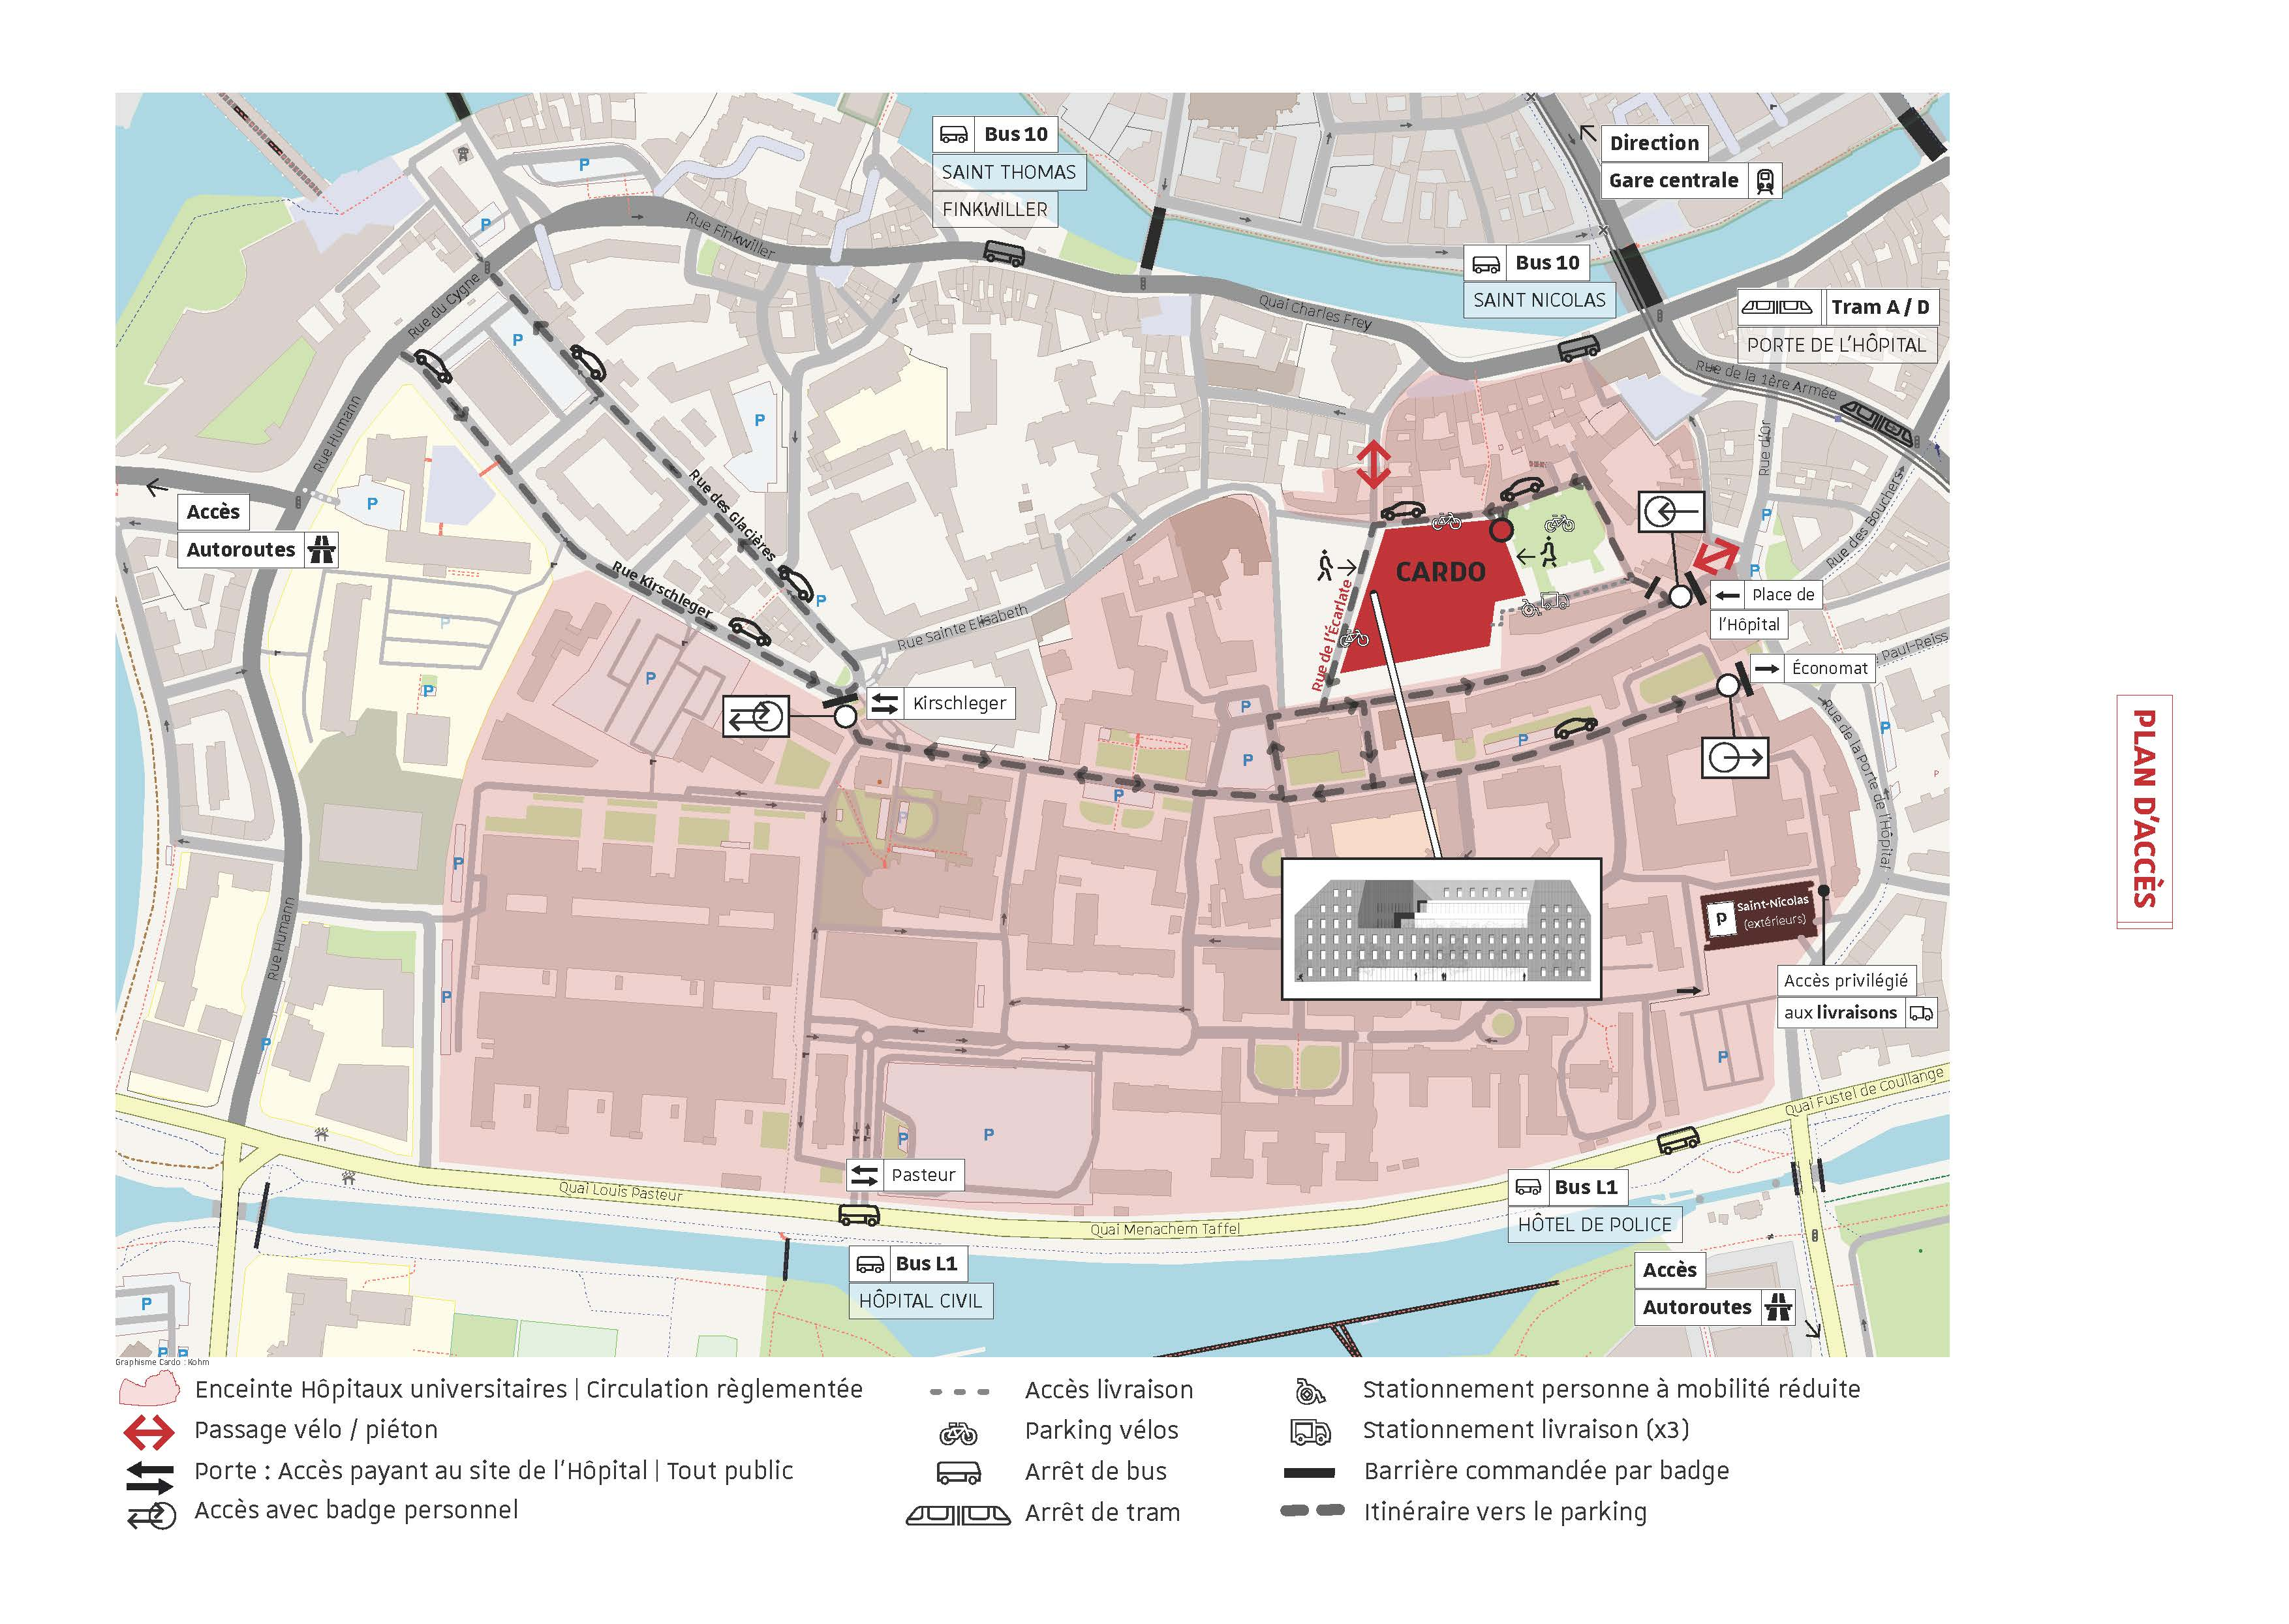
\includegraphics[width=0.8\linewidth]{images/Location_du_CEIPI} 

}

\caption{Location du CEIPI}(\#fig:Location du CEIPI)
\end{figure}

\hypertarget{la-structure}{%
\section{La structure}\label{la-structure}}

Le centre était composé de trois sections :
La section française dispense aux spécialistes français un enseignement en matière de propriété intellectuelle à l'échelle nationale et internationale.

La section internationale consacre son programme de formation au contrat de licence et s'adressait aux spécialistes français et étrangers, désirant acquérir des connaissances nécessaires de droit international.

Le laboratoire de Recherche du CEIPI, créé en 2006, sa dénomination officielle est UR 4375-Laboratoire de recherche du CEIPI. Il coordonne des activités variées pour la mission de réflexion quant à l'évolution du droit de la propriété intellectuelle dans la société de la connaissance.

Plus des informations sur le site du CEIPI :\url{https://www.ceipi.edu/}

\hypertarget{Sujet}{%
\chapter{Le sujet du stage}\label{Sujet}}

Le sujet de mon stage est quantification les évolutions législatives, en particulière pour les évolutions de la propriété intellectuelle. Les données pertinentes seront utilisées dans les recherches du CEIPI.

\hypertarget{douxf9-viennent-les-donnuxe9es}{%
\section{D'où viennent les données}\label{douxf9-viennent-les-donnuxe9es}}

Il existe trois dépôts git présentent les données législatives françaises :
\textbf{Legifrance} : \url{https://github.com/legifrance}

\textbf{Etalab} : \url{https://github.com/etalab/codes-juridiques-francais}

\textbf{Archeo Lex}: \url{https://archeo-lex.fr/}

Nous avons finalement choisi Archeo Lex. Bien que ses données ne soient pas aussi précises qu'EtabLab, mais il régulièrement mis à jour les données. En plus, ses données sont organisées bien, chaque code est placé dans un fichier séparé et nous pouvons trouver toutes les versions dans l'ordre.

\begin{figure}

{\centering \includegraphics{images/archeolex_structure} 

}

\caption{Les données dans Archeo Lex}\label{fig:ArcheoLex}
\end{figure}

\hypertarget{traitement-du-sujet}{%
\section{Traitement du sujet}\label{traitement-du-sujet}}

Après discussion, le stage a été divisé en deux parties.
L'un est l'exploration de données, dont le but est de créer une application qui peuvent générer des documents csv différentes en modifiant la ligne de commande.

L'autre est la visualisation des données.

\hypertarget{choix-des-outils}{%
\section{Choix des outils}\label{choix-des-outils}}

\hypertarget{langage}{%
\subsection{Langage}\label{langage}}

1.\textbf{Python} : nous avons choisi python comme langage d'exploration de données, car il contient de nombreux packages pouvant être appelés et il n'est pas difficile à apprendre.
Parmi eux, le package le plus important que nous utilisons est git-python*, qui peut être utilisé pour

2.\textbf{R et Rmd}: Nous avons choisi R comme langage de dessin. tidyverse, ggraphe et igraphe sont les plus fréquemment utilisés parmi les nombreux packages du langage R. La partie de code de R est stockée sous la forme d'un fichier Rmd, et le rapport que vous en train de lire et la diapositive de la soutenance sont tous générés par le fichier Rmd.

\hypertarget{ide}{%
\subsection{IDE}\label{ide}}

1.\textbf{Vscode} : l'outil d'environnement de développement le plus populaire. Il est très flexible et il est aussi techniquement abouti et très stable, je l'ai utilisé pour développer l'application python.

2.\textbf{Rstudio}: un environnement de développement gratuit, libre et multiplateforme pour R.il sert au traitement de données et à l'analyse statistique

\hypertarget{Application}{%
\chapter{Application archeolex\_excavation.py}\label{Application}}

\hypertarget{pruxe9sentation-guxe9nuxe9rale}{%
\section{Présentation Générale}\label{pruxe9sentation-guxe9nuxe9rale}}

\textbf{Rôle} : archeolex\_excavation.py est utilisée pour fouiller des dépôts git Archéo Lex et générer des fichiers csv. Nous pouvons générer différents fichiers csv en modifiant les paramètres dans la ligne de commande.

\textbf{Usage} : archeolex\_excavation.py {[}-h{]} {[}-d YYYY-MM-DD{]} {[}-f fichier.csv{]} {[}-t{]} {[}-v{]} diff\textbar check\textbar{} \textbar stats {[}code \ldots{]}

\textbf{Example}:

\begin{Shaded}
\begin{Highlighting}[]
\NormalTok{archeolex\_excavation.py stats code\_civil }\SpecialCharTok{{-}}\NormalTok{d last }\SpecialCharTok{{-}}\NormalTok{t }\SpecialCharTok{{-}}\NormalTok{s1 }\SpecialCharTok{{-}}\NormalTok{f test.csv}
\end{Highlighting}
\end{Shaded}

\hypertarget{les-paramuxe8tres}{%
\subsection{Les paramètres}\label{les-paramuxe8tres}}

\hypertarget{positional-arguments}{%
\subsubsection{Positional arguments}\label{positional-arguments}}

\begin{longtable}[]{@{}
  >{\raggedright\arraybackslash}p{(\columnwidth - 2\tabcolsep) * \real{0.50}}
  >{\raggedright\arraybackslash}p{(\columnwidth - 2\tabcolsep) * \real{0.50}}@{}}
\toprule
nom de paramètre & signification \\
\midrule
\endhead
\textbf{diff/check/status } & \textbf{Le traitement à effectuer} \\
diff & obtenir les informations de modification par article \\
check & détecter des erreurs des codes \\
status & Les informations de sous-section d'une section, ainsi que le nombre de lignes et de mots dans cette section.Les paramètres d'entrée -s1 à -s6 (voir ci-dessous) pour confirmer le niveau de cette section. \\
\textbf{codes } & \textbf{La liste des codes à fouiller} \\
\bottomrule
\end{longtable}

\hypertarget{les-niveaus-guxe9nuxe9raux-de-la-structure-des-codes}{%
\paragraph{Les niveaus généraux de la structure des codes}\label{les-niveaus-guxe9nuxe9raux-de-la-structure-des-codes}}

Partie

Sous\_partie

Livre

Titre

Chapitre

\hypertarget{optional-arguments}{%
\subsubsection{Optional arguments}\label{optional-arguments}}

\begin{longtable}[]{@{}
  >{\raggedright\arraybackslash}p{(\columnwidth - 2\tabcolsep) * \real{0.50}}
  >{\raggedright\arraybackslash}p{(\columnwidth - 2\tabcolsep) * \real{0.50}}@{}}
\toprule
nom de paramètre & signification \\
\midrule
\endhead
-h, --help & montrer le message de help et quitter \\
-d YYYY-MM-DD, --datelimit YYYY-MM-DD & définir une date maximum pour la fouille \\
-f nom.csv, --file nom.csv & écrit les données dans ce fichier csv (sortie standard par défaut) \\
-t, --fulltext & détecter les noms entiers des section \\
-s1 & Obtenir les informations de chaque chapitre \\
-s2 & Obtenir les informations de chaque livre \\
-s3 & Obtenir les informations de chaque titre \\
-s4 & Obtenir les informations de chaque sous partie \\
-s5 & Obtenir les informations de chaque partie \\
-s6 & Obtenir les informations de chaque code \\
\bottomrule
\end{longtable}

\hypertarget{quelques-fichies-csv-guxe9nuxe9ruxe9s}{%
\subsubsection{Quelques fichies csv générés}\label{quelques-fichies-csv-guxe9nuxe9ruxe9s}}

\hypertarget{example-1}{%
\paragraph{Example 1:}\label{example-1}}

\begin{figure}

{\centering 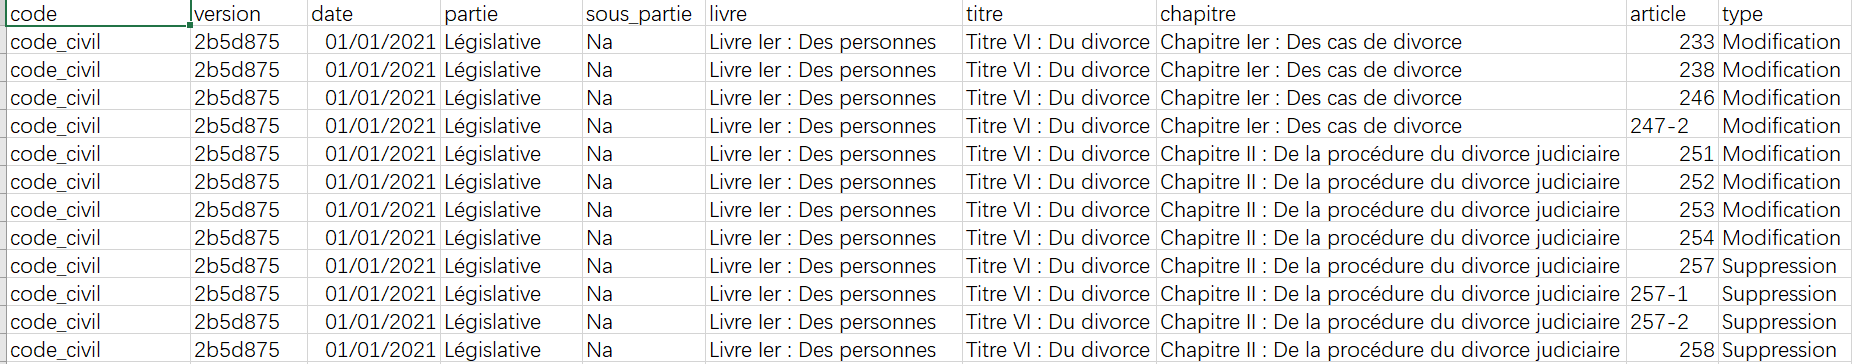
\includegraphics[width=0.8\linewidth]{images/diff} 

}

\caption{les informations de modification par article}\label{fig:diff}
\end{figure}

\hypertarget{example-2}{%
\paragraph{Example 2:}\label{example-2}}

L'application permet de détecter des erreurs de deux types :

\begin{itemize}
\tightlist
\item
  doublon : articles apparaissant deux fois dans un code ;
\item
  inversion : deux articles consécutifs dont la numérotation n'est pas croissante.
  Cette détection d'erreur est imparfaite, et n'exclu ni faux-positifs ni faux-négatifs. La date correspond à la version la plus ancienne à laquelle l'erreur a été détectée.
\end{itemize}

Les erreurs détectées sur un échantillon de codes se trouvent dans le fichier errors.csv, au format suivant :

\begin{figure}

{\centering 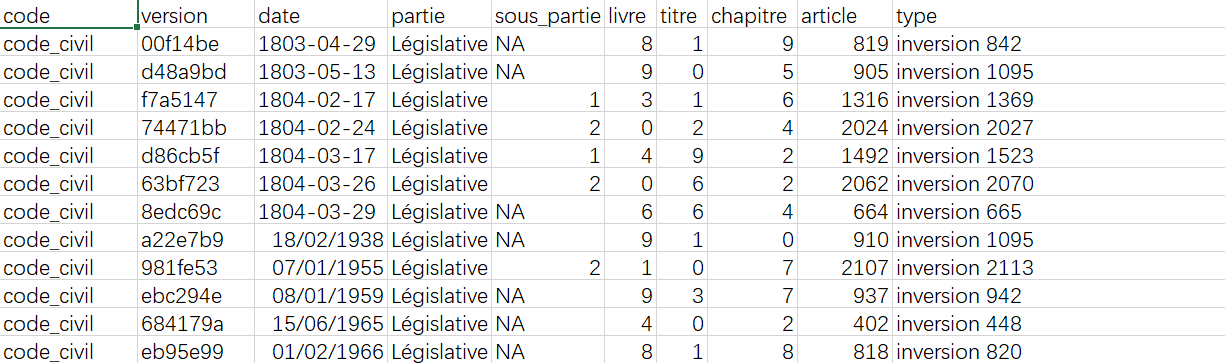
\includegraphics[width=0.8\linewidth]{images/check} 

}

\caption{détecter des erreurs des codes}\label{fig:check}
\end{figure}

\hypertarget{example-3}{%
\paragraph{Example 3}\label{example-3}}

\begin{figure}

{\centering 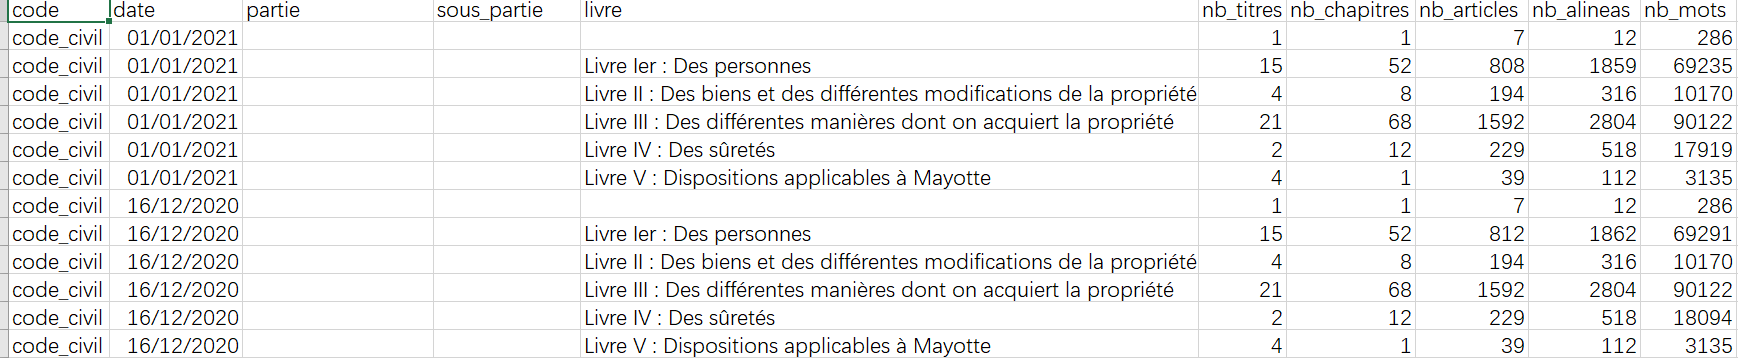
\includegraphics[width=0.8\linewidth]{images/stats3} 

}

\caption{Les informations de sous-section des livres, ainsi que le nombre de lignes et de mots pour chaque livres.}\label{fig:stats3}
\end{figure}

\hypertarget{example-4}{%
\paragraph{Example 4}\label{example-4}}

\begin{figure}

{\centering 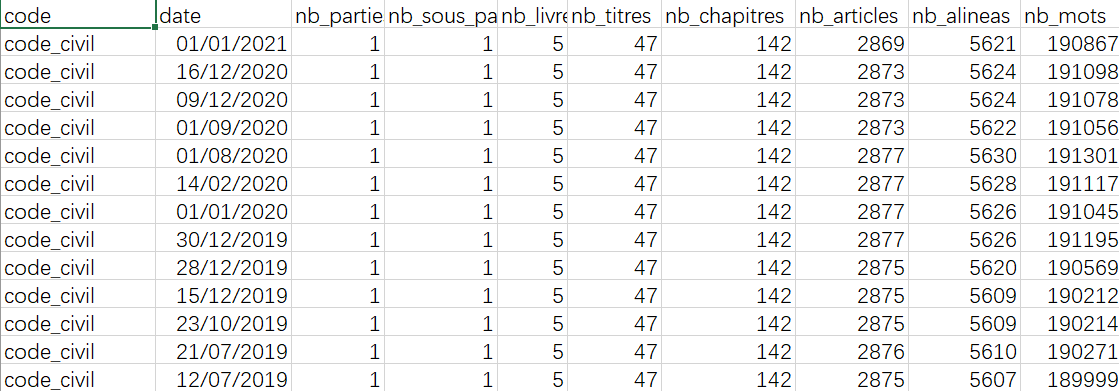
\includegraphics[width=0.8\linewidth]{images/stats6} 

}

\caption{Les informations de sous-section des chapitres, ainsi que le nombre de lignes et de mots pour chaque chapitre.}\label{fig:stats6}
\end{figure}

\hypertarget{pruxe9sentation-technique}{%
\section{Présentation technique}\label{pruxe9sentation-technique}}

\hypertarget{la-structure-des-codes}{%
\subsection{La structure des codes}\label{la-structure-des-codes}}

L'idée de code python est \textbf{orientée objet},il y a trois fichiers python:

1.\textbf{Article.py}: un article doit être considéré comme un objet, et les attributs liés à l'article peuvent être trouvés dans cette classe. Par exemple, le chapitre, le livre , le code où il se trouve, sa date, etc. (voir l'UML dans la figure ci-dessous pour plus de détails).
Les fonctions permettent de modifier ou d'obtenir la valeur des attributs d'article.

\begin{figure}

{\centering 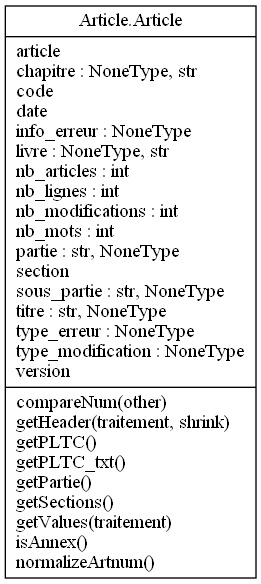
\includegraphics[width=0.25\linewidth]{images/Article_UML} 

}

\caption{le diagramme UML pour Article.py}\label{fig:Article}
\end{figure}

2.\textbf{ArcheoLexLog.py}:
Le rôle de cette classe est de stocker des fonctions d'exploration et d'analyse de données. Cette classe appelle la classe Article et appelle également un package très important GitPython* pour obtenir des informations de git diff.

\begin{figure}

{\centering 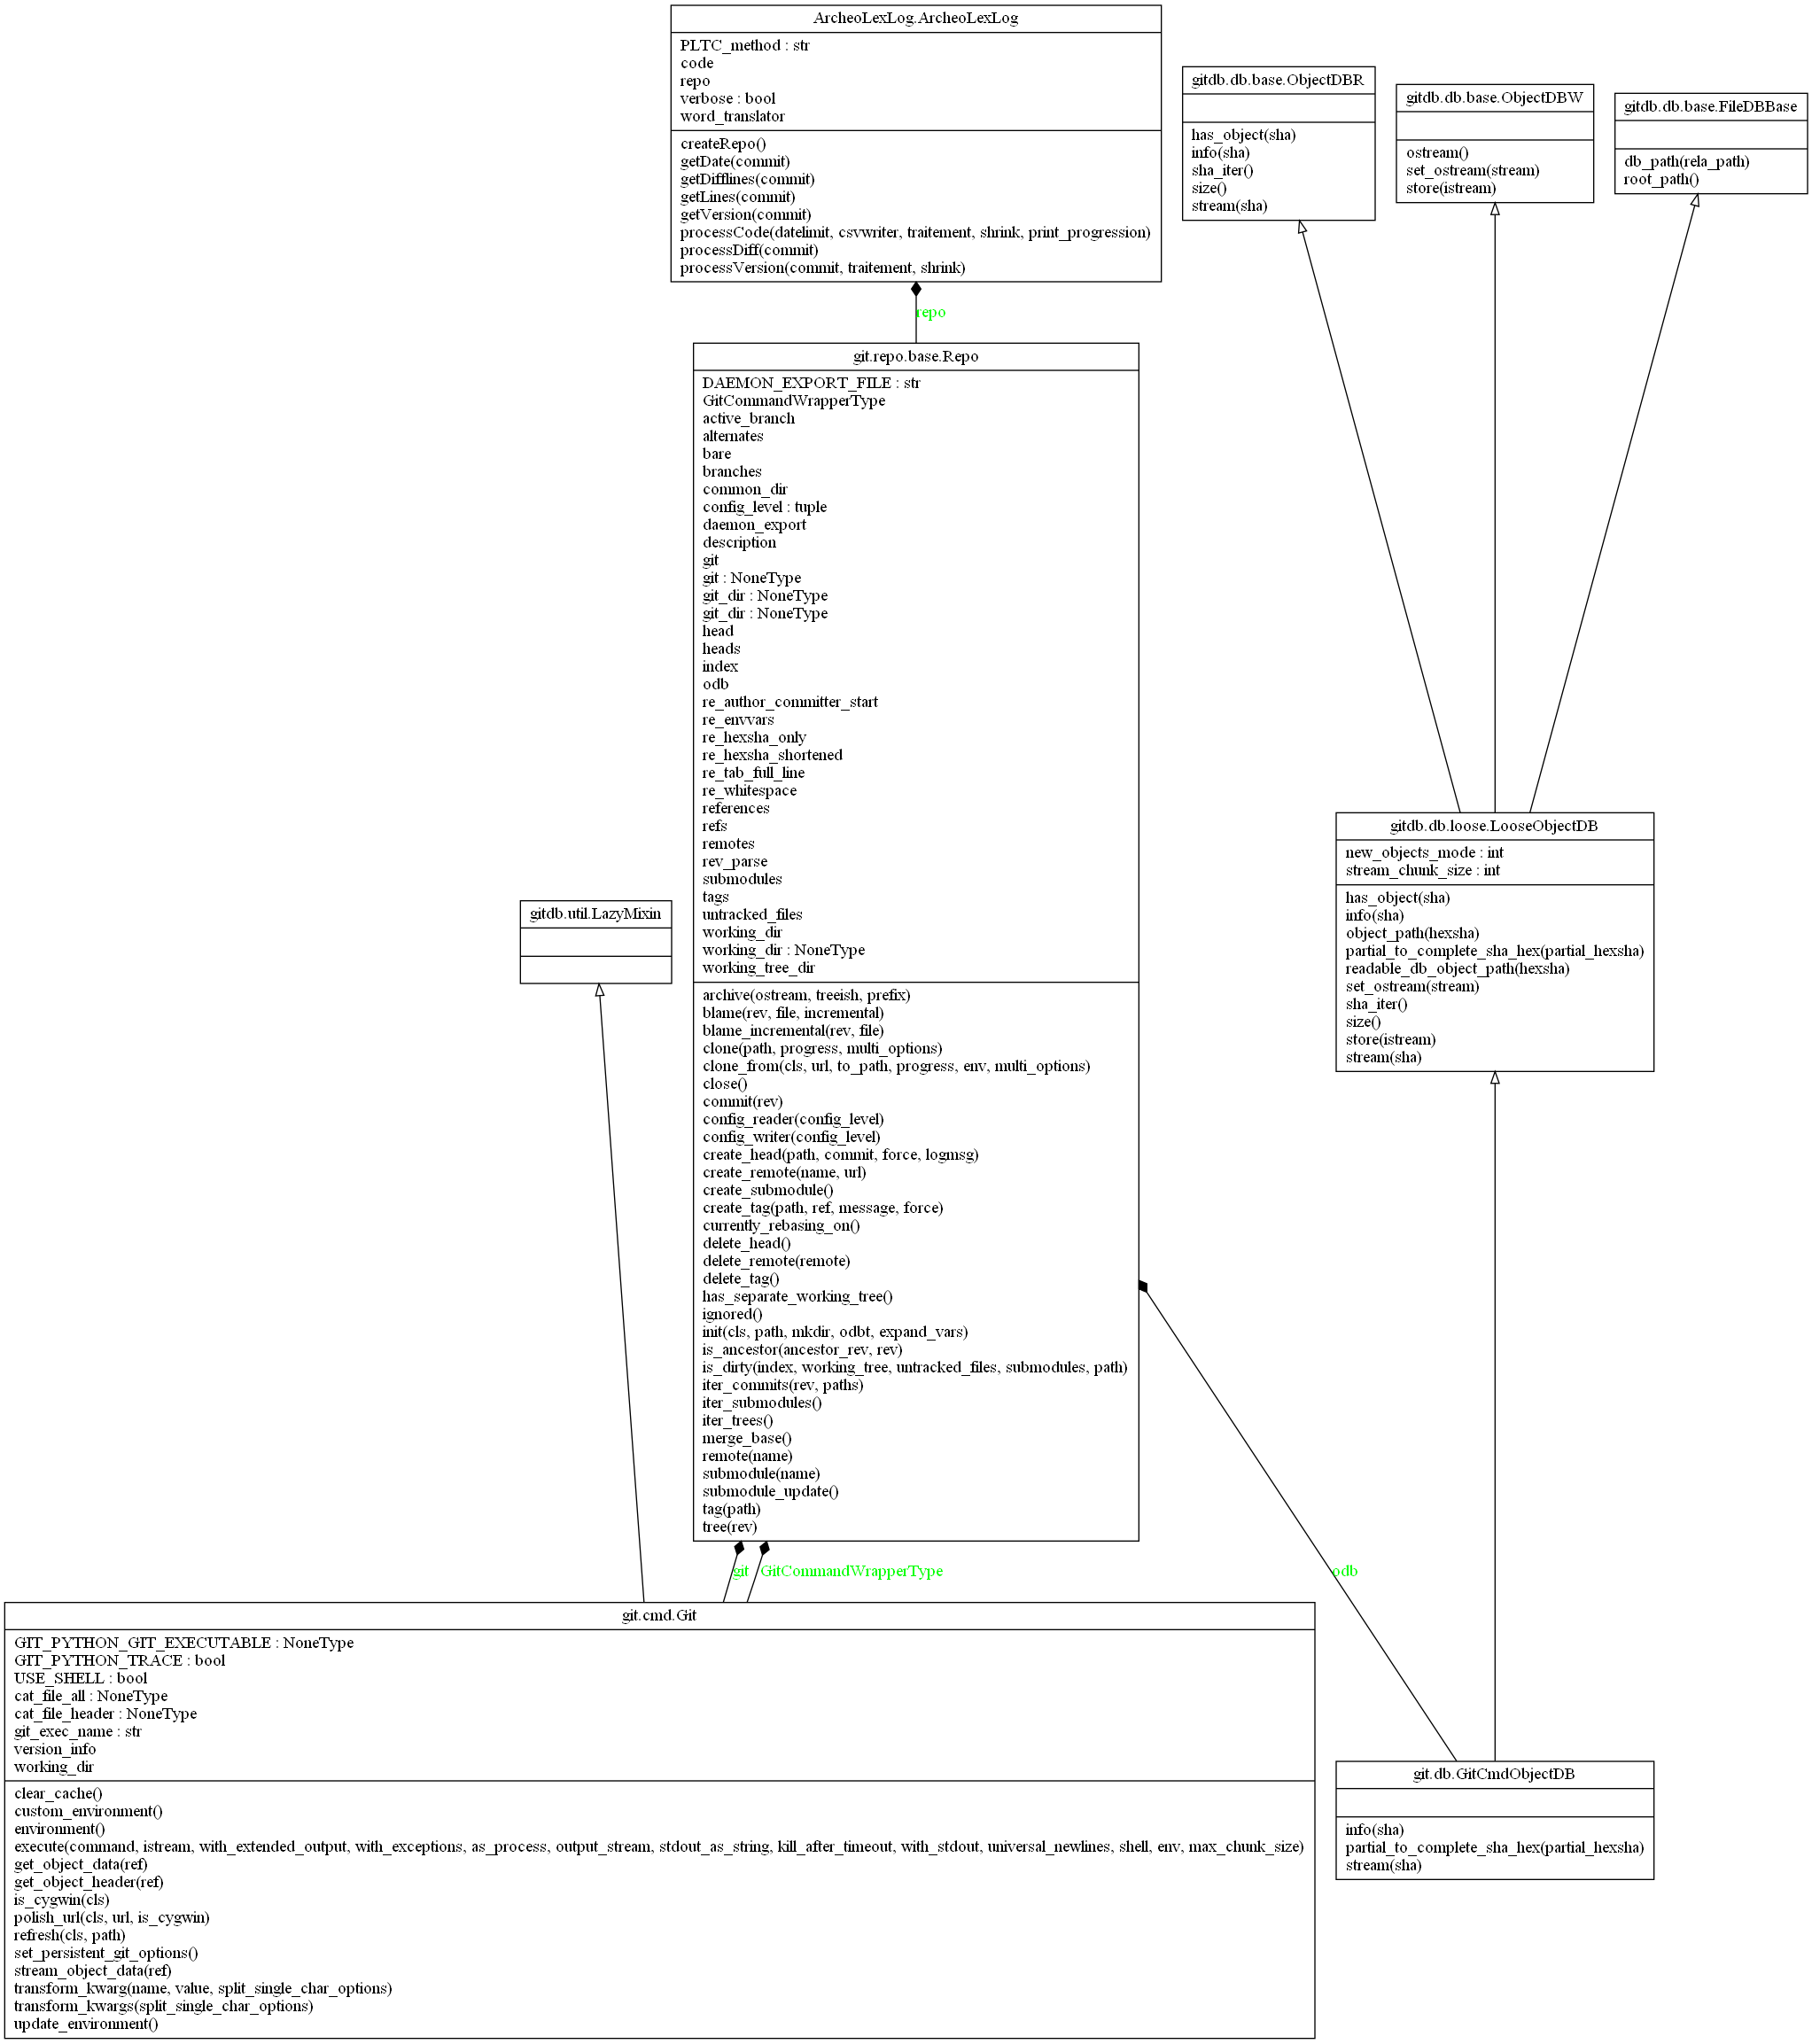
\includegraphics[width=1\linewidth]{images/ArcheoLexLog_UML} 

}

\caption{le diagramme UML pour ArcheoLexLog.py}\label{fig:ArcheoLexLog}
\end{figure}

3.\textbf{archeolex\_excavation.py}:Ce fichier appelle les deux classes Article et ArcheoLexLog, définit les paramètres et contient la fonction main.

\hypertarget{probluxe8mes-rencontruxe9s-et-solution}{%
\subsection{problèmes rencontrés et solution}\label{probluxe8mes-rencontruxe9s-et-solution}}

-1.Au début,l'idée était d'obtenir les informations de la structure de l'article à partir du nom. Par exemple : Article L312 -\textgreater{} L'article se trouve dans la partie législative, le troisième livre, le premier titre, le deuxième chapitre.
Cependant, il existe huit lois et leurs noms d'articles ne sont pas liés à la structure : code\_civil code\_de\_l'artisanat code\_de\_la\_famille\_et\_de\_l'aide\_sociale code\_de\_procédure\_civile code\_de\_procédure\_pénale code\_des\_postes\_et\_des\_communicet\_pélectroniquedemaraire\_demarale\_demarique

\textbf{Solution}: parcourir le texte complet du diff pour obtenir les informations de structure correspondantes. Et le nom complet(fulltext) de la structure est directement écrit dans la table sans utiliser le nom numérique.

-2.Un changement structurel après un commit. Par exemple: une nouvelle sous\_section est ajoutée

\textbf{Solution}: ajouter du code pour détecter et enregistrer ce changement.

-3.Les dépots git sur Archeo Lex ont des problème. Par exemple: il y a un problème avec l'ordre des articles, et le même article du même commit a été modifié plusieurs fois.

\textbf{Solution}: ajout d'un paramètre check pour détecter et afficher les erreurs, et envoyer les erreurs à Archeo Lex.

\hypertarget{final-words}{%
\chapter{Final Words}\label{final-words}}

We have finished a nice book.

  \bibliography{book.bib,packages.bib}

\end{document}
